\subsection{Winner Take All circuit}

A winner-take-all (WTA) circuit is a network of competing cells (neural,
software, or hardware) that reports only the response of the cell that has the strongest activation while suppressing the responses of all other cells. The circuit essentially implements a $max()$ function. These networks have been implemented in analog VLSI and applied to a wide variety of tasks, including selective attention, auditory localization, visual stereopsis, smooth pursuit/tracking, detection of heading direction and more. Today, it's a circuit that is basically everywhere. 

ADD FIGURE OF RESPONSE OF WTA

\paragraph{What's the biological basis behind Winner Take All?} It really is believed that populations of neurons do some kind of selective amplification to the broad range of input signals that they receive. Imagine you're at a loud cocktail party and there is a lot of noise but you suddenly hear your name being said, your brain will instantly cancel out everything else but the origin of the sound that you recognized as your name (localization and pitch/frequency of the voice). This is just one example. Anyways, in general, these circuits are typically used to implement and model competitive mechanisms among population of neurons. In this section we will analyze a class of WTA networks that emulate biological networks, consisting of a cluster of excitatory neurons that innervate a global feedback inhibitory neuron.


\begin{figure}[H]
    \centering
    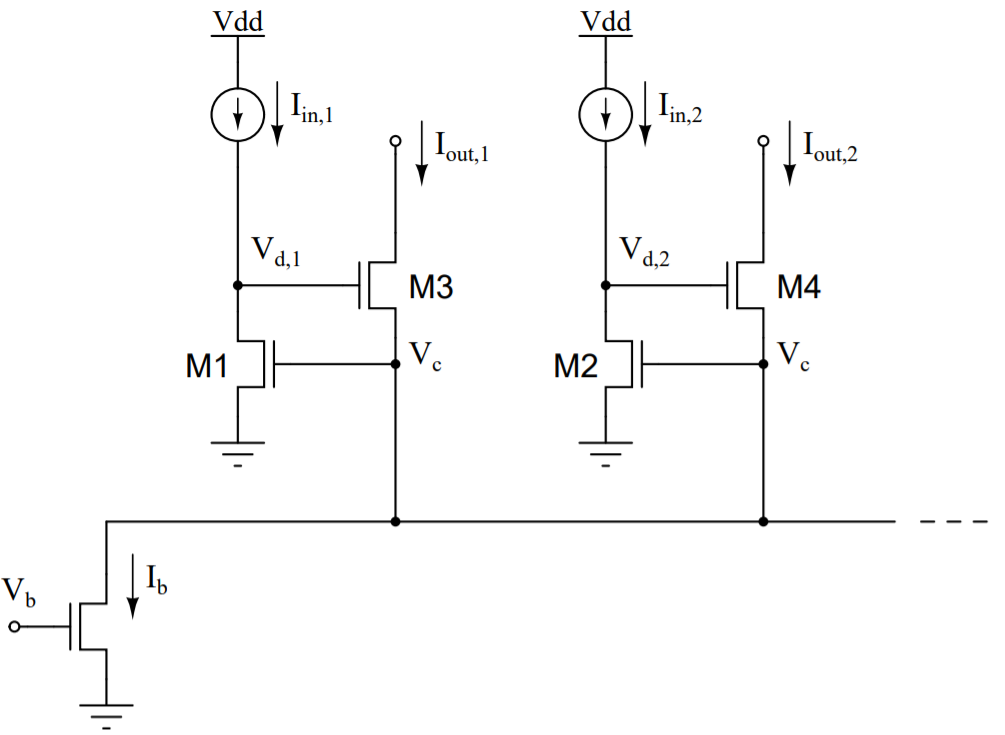
\includegraphics[width=0.6\linewidth]{../../Figures/Current_Mode_WTA.PNG}
    \caption{Current Mode Winner Take All. Adapted from Lecture.}
    \label{fig:Winner_Take_All}
\end{figure}

The circuit of Fig. \ref{fig:Winner_Take_All} is a continuous time, analog circuit that implements a WTA network. It processes all the (continuous-time) input signals in parallel, using only two transistors per input cell, and one global transistor that is common to all cells. Collective computation and global connectivity is obtained using one single node common to all cells. As can be seen in Fig. \ref{fig:Winner_Take_All}, each cell is built out of a current conveyor. The WTA network is modular and can be extended to N cells, by connecting additional cells to the node $V_c$. Input currents are applied to the network through current sources which are implemented for example using subthreshold pFETs. There are three conditions that determine the functionning of this WTA circuit, and we'll look at each of them individually. 

\subsubsection{$I_{in_1} = I_{in_2} = I_{in}$}

You should intuitively see (also from the previous normalizer circuit) that when $I_{in_1} = I_{in_2}$, $I_{out_1} = I_{out_2} = I_b/2$. Let's see how that works formally. First, from the current conveyor, we established that $V_c \propto \mathrm{ln}(I_{in})$, which if written formally gives: 

\begin{equation}
    V_c = \frac{U_T}{\kappa}\mathrm{ln}(\frac{I_{in_1}}{I_0})
\end{equation}

Because $I_{in_1} = I_{in_2}$, it follows that $V_d_1 = V_d_2$, which yields that $I_{out_1} = I_{out_2} = I_b/2$. As simple as that. 


To remember: 

\begin{itemize}
    \item $V_c = \frac{U_t}{\kappa}ln(\frac{I_{in}}{I_0})$
    \item $I_{out}_1 = I_{out}_2 = I_b$
    \item $V_d_1 = V_d_2 \approx V_c + V_b$
\end{itemize}


\subsubsection{$I_{in_1} \gg I_{in_2}$}

This is a bit trickier. We first need to recall from Chapter 2 and 3 that the subthreshold current flowing through a transistor can be divided into a \textit{forward} component, $I_f$ and a \textit{reverse} component, $I_r$. When the transistor’s source voltage $Vs$ is approximately equal to its drain voltage $Vd$ (so when we are in the Ohmic region), $I_r$ becomes comparable to $I_f$. Now let's just keep this property in mind and look at the circuit for the case where $I_{in_1} \gg I_{in_2}$.

When $I_{in_1} \gg I_{in_2}$, if the drain voltage of $M_1$ is in saturation, the dominant component of its drain current will be in the forward direction and its gate voltage $V_c$ will increase such that $I_d_1 = I_f_1 = I_0e^{\kappa V_c/U_T} = I_{in_1}$.  Although the two input currents $I_{in_1}$ and $I_{in_2}$ are different, the forward component of the drain currents of M1 and M2 are equal ($I_{f_1}= I_{f_2}$) because the two transistors
have a common gate voltage $V_c$, and both their sources are tied to ground. The drain current $I_d_2$ of transistor M2 can only be equal to the input current $I_{in_2}$ under the following conditions:

\begin{equation}
    I_f_2 - I_r_2 = I_{in_2}
\end{equation}
\begin{equation}
    \mathrm{which \ implies \ that: \ }I_r_2 = I_f_2 - I_{in_2}
\end{equation}
\begin{equation}
    \mathrm{which \ implies \ that: \ }I_r_2 = I_{in_1} - I_{in_2} >> 0
\end{equation}

The reverse component of $I_d_2$ becomes significant only if $V_d_2$ decreases
enough for $M_2$ to operate in its ohmic region. In this case, the output transistor $M4$ is effectively switched off, and $I_{out_2} = 0$. Consequently,
$M3$ sources all the bias current ($I_{out_1} = Ib$), with $V_d_1$ satisfying the equation $I_b = I_0e^{\kappa V_d_1 - Vc}$. 

To remember: 

\begin{itemize}
    \item $V_c = \frac{U_t}{\kappa}ln(\frac{I_{in}_1}{I_0})$
    \item $I_{out}_1 = I_b; \ I_{out}_2 = 0$
    \item $V_d_1 = V_c + V_b$
    \item $V_d_2 \approx 0$
\end{itemize}

Typical $\delta V$ that make this condition apply are actually as small as ~5mV. It's only when $\delta V$ is smaller than this that we are in the operating regime described below.  

\subsubsection{$I_{in_1} = I_{in_2} \pm \delta I_{in}$}

To analyze the circuit in this regime, we must consider the Early effect of the transistor operating in the saturation region. Recall that considering the Early Effect, current in a transistor in saturation is: 

\begin{equation}
    I_{ds} = I_{sat}(1 + \frac{V_{ds}}{V_e})
\end{equation}
where $V_e$ is the early voltage. 

Assume that the two input currents $I_{in_1}$ and $I_{in_2}$ are initially equal. In this case, the transistors $M_1$ and $M_2$ operate in saturation region: the output voltages $V_d_1$ and $V_d_2$ will settle to a common value and the output currents $I_{out_1}$ and $I_{out_2}$ are both equal to $I_b/2$ as established previously. If we now increase the input current $I_{in_1}$ by a small amount $\delta_I$ and apply the previous equation to transistor $M_1$, then the drain voltage $V_d_1$ increases by: 

\begin{equation}
    \delta V = \frac{\delta I}{I_{sat}}V_e
\end{equation}

As $V_d_1$ is also the gate voltage of transistor $M_3$, the $I_{out_1}$ will be amplified by an amount proportional to $e^{\delta V}$. The constraint of Kirchoff's current law imposes that $I_{out_2}$ decreases by the same amount in steady state. This reduction means that gate voltage $V_d_2$ of $M_4$ must decrease by $\delta V$. 

The gain of the competition mechanism $\frac{\delta V}{\detla I}$ in the small signal regime is directly proportional to the Early voltage and inversely proportional to $I_{sat}$. The Early voltage depends on the geometry of the transistors and is fixed at design time. On the other hand $I_{sat}$ depends on $V_c$, which changes with the amplitude of the input currents. 

To remember: 

\begin{itemize}
    \item $I_{ds} = I_{sat}(1 + \frac{V_{ds}}{V_e})$
    \item $V_d_2 = V_d_1 - V_e \frac{\delta I}{I_{sat}}$
    \item $I_{out}_2 < I_{out}_1$
\end{itemize}

\subsubsection{Experimental data}

We can see experimental data on figure \ref{fig:WTA_Output}. 

\begin{figure}[H]
    \centering
    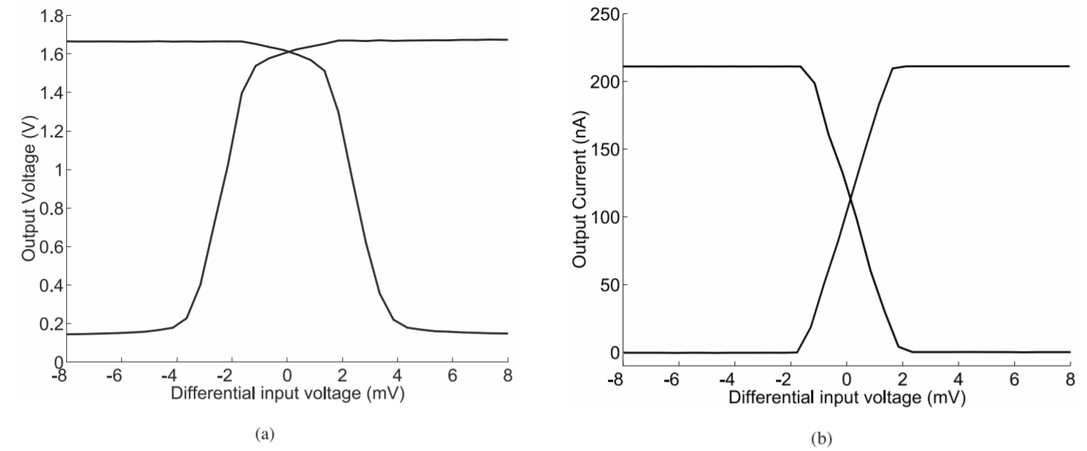
\includegraphics[width=0.9\linewidth]{../../Figures/WTA_Output.PNG}
    \caption{Responses of the current conveyor two-cell WTA circuit. a) Voltage output ($V_d_1$ and $V_d_2$) versus the differential input voltage. (b) Current output ($I_{out_1}$ and $I_{out_2}$). The bias voltage $V_b$ = 0.7V. The small difference in the maximum output currents is due to device mismatch effects in the read-out transistors of the two cells. Adapted from textbook.}
    \label{fig:WTA_Output}
\end{figure}

We can see the output voltages ($V_d_1$ and $V_d_2$) and output currents ($I_{out}_1$ and $I_{out}_2$) of the circuit, in response to the differential input voltage $\delta V$ which encodes the ratio of the input currents that were provided by pFETs operating in subthreshod. $V_{in}_1$ was set to 4.3$V$ while the gate voltage of the input current pFET $V_{in}_2$ was set to $V_{in}_2 = V_{in}_1 + \delta V$, thereby allowing to test all different three case scenarios by changing $\delta V$. We can clearly see that experimental result go well with our theoretical findings!

















